\documentclass[aspectratio=169]{beamer}

\mode<presentation>
{
  \usetheme{default}
  \usecolortheme{default}
  \usefonttheme{default}
  \setbeamertemplate{navigation symbols}{}
  \setbeamertemplate{caption}[numbered]
  \setbeamertemplate{footline}[frame number]  % or "page number"
  \setbeamercolor{frametitle}{fg=white}
  \setbeamercolor{footline}{fg=black}
} 

\usepackage[english]{babel}
\usepackage[utf8x]{inputenc}
\usepackage{tikz}
\usepackage{courier}
\usepackage{array}
\usepackage{bold-extra}
\usepackage{minted}
\usepackage[thicklines]{cancel}

\xdefinecolor{dianablue}{rgb}{0.18,0.24,0.31}
\xdefinecolor{darkblue}{rgb}{0.1,0.1,0.7}
\xdefinecolor{darkgreen}{rgb}{0,0.5,0}
\xdefinecolor{darkgrey}{rgb}{0.35,0.35,0.35}
\xdefinecolor{darkorange}{rgb}{0.8,0.5,0}
\xdefinecolor{darkred}{rgb}{0.7,0,0}
\definecolor{darkgreen}{rgb}{0,0.6,0}
\definecolor{mauve}{rgb}{0.58,0,0.82}

\title[2017-10-13-lpc-testdrive]{New software for offline analysis}
\author{Jim Pivarski}
\institute{Princeton University -- DIANA}
\date{October 13, 2017}

\begin{document}

\logo{\pgfputat{\pgfxy(0.11, 7.4)}{\pgfbox[right,base]{\tikz{\filldraw[fill=dianablue, draw=none] (0 cm, 0 cm) rectangle (50 cm, 1 cm);}
\includegraphics[height=1 cm]{diana-hep-logo.png}}}}

\begin{frame}
  \titlepage
\end{frame}

% Uncomment these lines for an automatically generated outline.
%\begin{frame}{Outline}
%  \tableofcontents
%\end{frame}

%%%%%%%%%%%%%%%%%%%%%%%%%%%%%%%%%%%%%%%%%%%%%%%%%%%%%%%

%%%% START

%% \begin{frame}{Purpose of this talk}
%% \vspace{0.15 cm}
%% \begin{center}
%% \large To show you some of the software packages I've been developing \underline{so you can use them} and either get more productive or send me critical feedback.

%% \vspace{1 cm}
%% \uncover<2->{(I'm looking for beta testers.)}
%% \end{center}
%% \end{frame}

%% \begin{frame}{What is the software for?}
%% \vspace{0.15 cm}
%% \large Ultimately, I and several others\footnote{Oliver Gutsche, Igor Mandrichenko (FNAL), Tanu Malik (DePaul CS), \mbox{Jean-Roch Vlimant (CalTech),\hspace{-1 cm}} Manos Karpathiotakis, Miguel Branco, Ioannis Alagiannis, Anastasia Ailamaki (EPFL/ATLAS)\ldots} want to develop a centralized service that will respond to requests for plots more rapidly than local skims.

%% \vspace{0.5 cm}
%% \uncover<2->{The trick is to make it respond quickly enough that you'll use it.}

%% \vspace{0.5 cm}
%% \uncover<3->{We're still at the stage of studying the scaling behaviors of various options, but meanwhile, I've been developing fast data access methods that you can use now, independently of any query system.}

%% \vspace{0.5 cm}
%% \uncover<4->{You can\ldots\ er\ldots\ use it on your skims.}
%% \end{frame}

%% \begin{frame}[fragile]{Experiment to try sometime}
%% \vspace{0.25 cm}
%% \textcolor{darkblue}{How long \underline{should} it take to compute something?}

%% \small
%% \begin{minted}{python}
%% from time import *
%% from numpy import *

%% pt1 = random.normal(0, 1, int(1e6))**2
%% eta1 = random.uniform(-5, 5, int(1e6))
%% phi1 = random.uniform(-5, 5, int(1e6))

%% pt2 = random.normal(0, 1, int(1e6))**2
%% eta2 = random.uniform(-5, 5, int(1e6))
%% phi2 = random.uniform(-5, 5, int(1e6))

%% start = time()
%% mass = sqrt(2*pt1*pt2*(cosh(eta1 - eta2) - cos(phi1 - phi2)))
%% end = time()

%% print(end - start)
%% \end{minted}

%% \normalsize
%% \vspace{-6 cm}\hfill\begin{minipage}{0.35\linewidth}
%% \begin{uncoverenv}<2->
%% \begin{center}
%% \textcolor{darkblue}{$10^6$~events / 0.24 sec = 4.16~MHz}

%% \vspace{0.25 cm}
%% We need to get used to numbers like this.
%% \end{center}
%% \end{uncoverenv}
%% \vspace{6 cm}
%% \end{minipage}
%% \end{frame}

%% \begin{frame}[fragile]{Experiment to try sometime: hardcore version}
%% \vspace{0.1 cm}
%% \scriptsize
%% \begin{minted}{python}
%% import ctypes
%% import os

%% open("little-c-function.c", "w").write("""
%% #include "math.h"

%% void computemass(double* pt1, double* eta1, double* phi1,
%%                  double* pt2, double* eta2, double* phi2,
%%                  double* mass) {
%%   int i;
%%   for (i = 0;  i < (int)1e6;  i++)
%%     mass[i] = sqrt(2*pt1[i]*pt2[i]*(cosh(eta1[i] - eta2[i]) - cos(phi1[i] - phi2[i])));
%% }
%% """)
%% os.system("gcc -O3 -shared -fPIC little-c-function.c -o little-c-function.so")

%% computemass = ctypes.cdll.LoadLibrary("little-c-function.so").computemass
%% output = numpy.empty(int(1e6))

%% start = time()
%% computemass(*[x.ctypes.data_as(ctypes.POINTER(ctypes.c_double))
%%                                    for x in pt1, eta1, phi1, pt2, eta2, phi2, output])
%% end = time()

%% print(end - start)
%% \end{minted}
%% \normalsize
%% \vspace{-8 cm}\hfill\begin{minipage}{0.35\linewidth}
%% \begin{uncoverenv}<2->
%% \begin{center}
%% Not much faster:

%% \textcolor{darkblue}{$10^6$~events / 0.203 sec = 4.9~MHz}
%% \end{center}
%% \end{uncoverenv}
%% \vspace{8 cm}
%% \end{minipage}
%% \end{frame}

%% \begin{frame}{}
%% \vspace{1 cm}
%% \begin{center}
%% \large If you're computing masses considerably slower than 5~million per second, most of your computer's time is spent doing something other than physics.
%% \end{center}

%% \vspace{0.5 cm}
%% \begin{itemize}
%% \item<2-> Usually, it's for a very good reason: managing complexity.
%% \item<3-> You'll notice that I set up those examples in Python. Python is one of the slowest languages available. It spends most of its time presenting a simple data model and a safe environment to the user (me).
%% \item<4-> But when you've got your task expressed in mathematical form, you'd like it to spend all of its time computing.
%% \end{itemize}
%% \end{frame}

\begin{frame}{Bypassing ROOT's TTree::GetEntry}
\vspace{0.5 cm}
ROOT data are stored in an efficient format--- arrays similar to the Numpy example on the previous page.

\vspace{1 cm}
\uncover<2->{But pieces of each array are spliced into local variables each time {\tt GetEntry} is called. (Also, it's fairly complex, thwarts vectorization, virtual function calls\ldots)}

\vspace{1 cm}
\uncover<3->{Accessing the data without {\tt GetEntry} (which includes {\tt TTree::Draw}!) is an order of magnitude faster. We're adding a method to ROOT 6.12 (next version) to dump data directly into Numpy arrays.}
\end{frame}

\begin{frame}{Illustration using NanoAOD decompression rate studies}
\begin{center}
\textcolor{darkblue}{\large Hint: vertical scale on right is 30$\times$ higher, reaches 0.5~MHz}
\end{center}

\begin{columns}
\column{0.45\linewidth}
\mbox{ } \hfill Reading through {\tt GetEntry} \hfill \mbox{ }

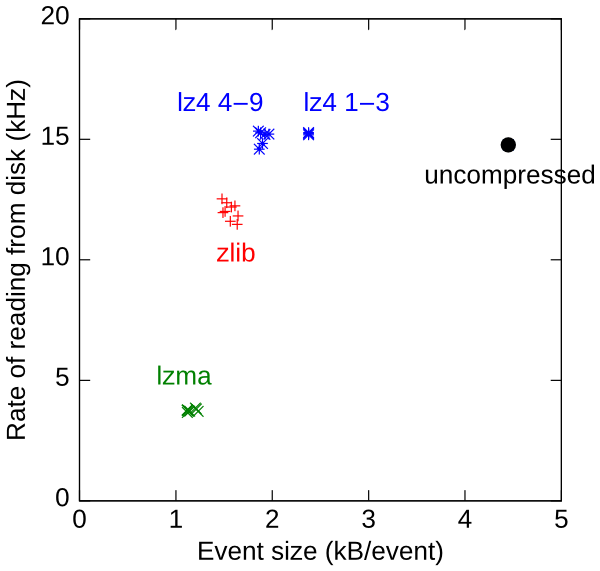
\includegraphics[width=\linewidth]{read.png}

\column{0.45\linewidth}
\mbox{ } \hfill New ROOT-to-Numpy method \hfill \mbox{ }

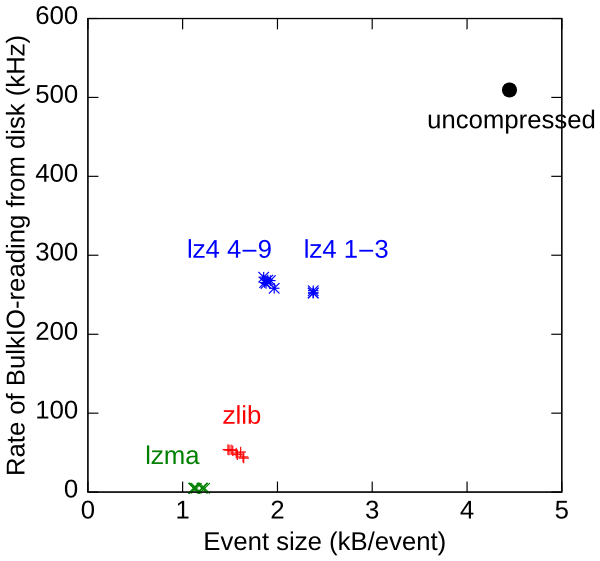
\includegraphics[width=\linewidth]{bulk.png}

\end{columns}
\end{frame}

\begin{frame}{ROOT 6.12 isn't out yet\ldots}
\vspace{0.5 cm}
So I wrote this access method in pure Python+Numpy:

\begin{center}
\href{https://github.com/scikit-hep/uproot}{\textcolor{blue}{\Large https://github.com/scikit-hep/uproot}}
\end{center}

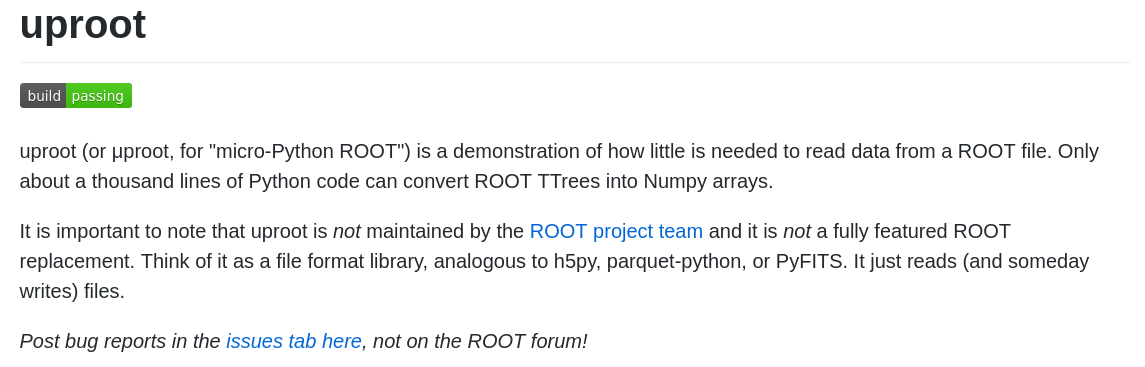
\includegraphics[width=\linewidth]{uproot.png}

\begin{center}
\Large \textcolor{red}{\tt pip install uproot --user}
\end{center}
\end{frame}

\begin{frame}{But\ldots\ Python is slow\ldots\ why Python???}
\vspace{0.4 cm}
{\large If you're reading a reasonably large file (GB+), most of the time is spent in a Numpy call, not Python.}

\vspace{0.3 cm}
\begin{uncoverenv}<2->
\begin{tabular}{l c c c}
& \underline{Time to open file}$^{\mbox{\scriptsize *}}$ & & \\
C++/{\tt GetEntry} & 0.50 sec & & \\
Python/uproot & 0.03 sec & & \\
& & & \\
 & \underline{Time to read file} & \underline{Event rate} & \underline{Data rate} \\
C++/{\tt GetEntry} & 4.62 sec & 1.9 MHz & \textcolor{white}{0}230 MB/sec \\
Python/uproot & 0.93 sec & 9.2 MHz & 1160 MB/sec \\
& & & \\
& \underline{Time to read 1 branch} & \underline{Event rate} & \underline{Data rate} \\
C++/{\tt GetEntry} & 0.256 sec & \textcolor{white}{0}33 MHz & \textcolor{white}{0}260 MB/sec \\
Python/uproot & 0.064 sec & 133 MHz & 1020 MB/sec
\end{tabular}

\vspace{0.5 cm}
{\scriptsize $^{\mbox{\scriptsize *}}$from \href{https://indico.cern.ch/event/567550/contributions/2628878/}{\textcolor{blue}{Jakob Blomer's 2017 ACAT talk}} about ROOT performance, 1 GB uncompressed, flat table from LHCb.}
\end{uncoverenv}

\vspace{-6.1 cm}\hfill\begin{minipage}{0.35\linewidth}
\begin{uncoverenv}<3->
\begin{center}
\large
\textcolor{darkblue}{about 5$\times$ faster}

\vspace{0.1 cm}
\textcolor{darkblue}{(rather than 30$\times$)}
\end{center}
\end{uncoverenv}
\vspace{6.1 cm}
\end{minipage}
\end{frame}

\begin{frame}{But\ldots\ Python can't be parallelized because of the GIL}
\vspace{0.4 cm}
{\large Python's Global Interpreter Lock (GIL) thwarts parallelization performance of Python statements, but external calls to Numpy release this lock.}

\vspace{0.35 cm}
\textcolor{darkblue}{uproot scales up to about 30 threads (Knight's Landing with 128 threads below).}

\vspace{0.35 cm}
\begin{columns}
\column{0.4\linewidth}
\mbox{ } \hfill scaling of whole-file reading \hfill \mbox{ }

\vspace{0.2 cm}
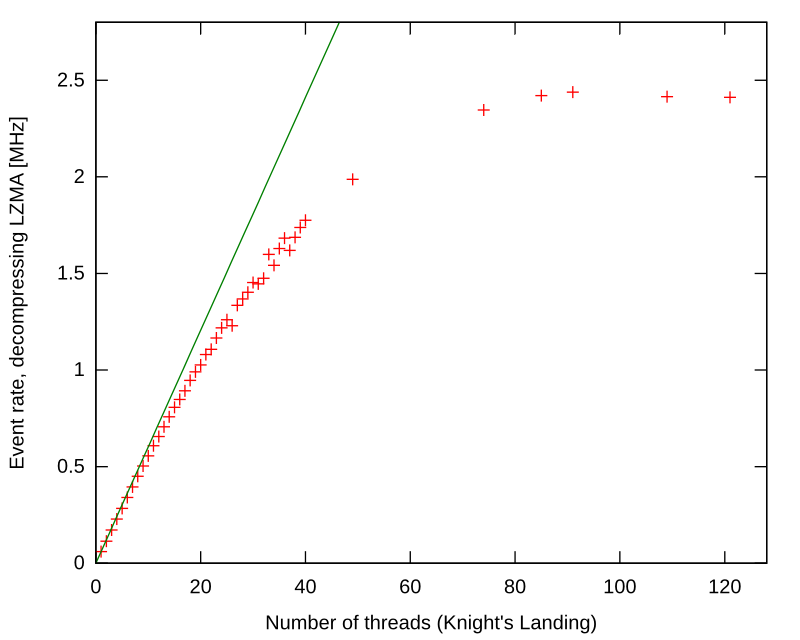
\includegraphics[width=\linewidth]{uproot-scaling.png}

\column{0.4\linewidth}
\mbox{ } \hfill scaling of single-branch reading \hfill \mbox{ }

\vspace{0.2 cm}
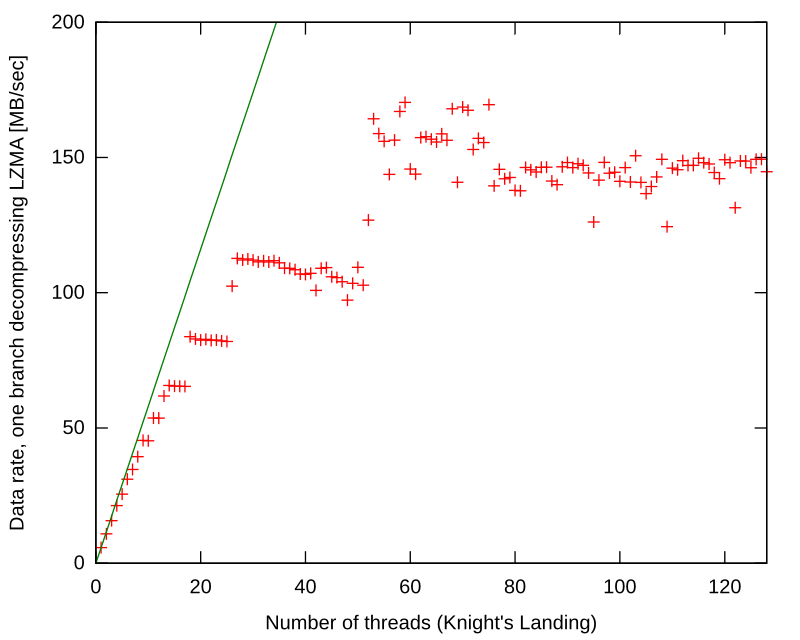
\includegraphics[width=\linewidth]{uproot-scaling-2.png}

\end{columns}
\end{frame}

\end{document}
